\documentclass[10pt,twocolumn]{article}

\usepackage[margin=0.9in,top=1in,bottom=1in]{geometry}
\usepackage{times}
\usepackage{hyperref}
\usepackage{graphicx}
\usepackage{booktabs}
\usepackage{listings}
\usepackage{xcolor}
\usepackage{amsmath}
\usepackage{amssymb}
\usepackage{algorithm}
\usepackage{algpseudocode}
\usepackage{subcaption}
\usepackage{multirow}
\usepackage{url}
\usepackage{microtype}
\usepackage{enumitem}
\usepackage{balance}
\usepackage{tikz}
\usepackage{pgfplots}
\pgfplotsset{compat=1.18}
\usetikzlibrary{shapes.geometric, arrows.meta, positioning, fit, backgrounds, calc}

%% ------------------------------------------------------------------
%% Color palette (monochrome-friendly for print)
%% ------------------------------------------------------------------
\definecolor{darkgray}{RGB}{50,50,50}
\definecolor{midgray}{RGB}{130,130,130}
\definecolor{lightgray}{RGB}{220,220,220}
\definecolor{accentblue}{RGB}{30,80,160}
\definecolor{codebackground}{RGB}{248,248,248}

\lstset{
  basicstyle=\ttfamily\scriptsize,
  keywordstyle=\color{accentblue}\bfseries,
  commentstyle=\color{midgray}\itshape,
  stringstyle=\color{darkgray},
  breaklines=true,
  backgroundcolor=\color{codebackground},
  frame=single,
  rulecolor=\color{lightgray},
  numbers=left,
  numberstyle=\tiny\color{midgray},
  xleftmargin=1.5em,
  framexleftmargin=1.5em,
  aboveskip=6pt,
  belowskip=6pt,
}

\hypersetup{
  colorlinks=true,
  linkcolor=accentblue,
  citecolor=accentblue,
  urlcolor=accentblue,
}

%% ------------------------------------------------------------------
%% TikZ styles
%% ------------------------------------------------------------------
\tikzset{
  box/.style={rectangle, rounded corners=4pt, draw=darkgray, thick,
              fill=white, text centered, minimum height=1.8em, minimum width=4.5em,
              font=\small},
  toolbox/.style={rectangle, rounded corners=2pt, draw=midgray,
                  fill=lightgray!50, text centered, minimum height=1.5em,
                  font=\scriptsize},
  phase/.style={rectangle, rounded corners=4pt, draw=darkgray, thick,
                fill=white, text centered, minimum height=2em, minimum width=5em,
                font=\small\bfseries},
  arrow/.style={-{Stealth[length=5pt]}, thick, draw=darkgray},
  dasharrow/.style={-{Stealth[length=5pt]}, dashed, draw=midgray},
}

%% ------------------------------------------------------------------
\title{%
  \textbf{CARA: A Contract-Aware Refactoring Agent\\for Distributed Systems}\\[0.4em]
  {\large Unified Schema and API Co-Evolution via LLM-Powered Tool Orchestration}%
}

\author{%
  Nikhil Katre\thanks{Equal contribution. Work performed independently of the authors' employers.}\\
  \textit{Independent Researcher}\\
  \texttt{npkatre@gmail.com}
  \and
  Shweta Mane\thanks{Equal contribution. Work performed independently of the authors' employers.}\\
  \textit{Google}\\
  \texttt{maneshweta1991@gmail.com}%
}

\date{March 2026}

\begin{document}
\maketitle

%% ------------------------------------------------------------------
\begin{abstract}
%% ------------------------------------------------------------------
Refactoring data models in distributed systems is one of the highest-risk
engineering activities in production software. When a schema changes, the
impact propagates across two tightly coupled but independently managed layers:
the \emph{storage layer} (SQL schemas, Protobuf definitions) and the
\emph{interface layer} (REST/OpenAPI contracts, gRPC service definitions).
Existing tools address each layer in isolation, forcing engineers to manually
coordinate migrations and creating a well-documented source of production incidents.

We present \textbf{CARA} (Contract-Aware Refactoring Agent), the first LLM-based
agent that treats schema evolution and API contract evolution as a \emph{unified
refactoring lifecycle}. CARA employs a ReAct reasoning loop~\cite{yao2023react}
over a seven-tool registry to simultaneously detect changes across both layers,
trace downstream consumers across service boundaries, classify every change as
\texttt{SAFE}, \texttt{BACKWARD\_COMPATIBLE}, or \texttt{BREAKING}, and generate
a coordinated expand-contract migration plan with tested adapter code in Python,
Java, Kotlin, and TypeScript.

We evaluate CARA on a 515-case benchmark (15 expert-crafted plus 500
programmatically generated from real-world patterns) spanning five change
categories. CARA achieves \textbf{0.86 F1} on breaking-change detection,
\textbf{1.00} expand-contract compliance, and \textbf{0.97} plan completeness,
outperforming both rule-based and prompt-only baselines by substantial margins.
Five repeated runs yield standard deviation 0.000 across all metrics,
confirming full reproducibility. All code, benchmark data, and evaluation
scripts are publicly available.
\end{abstract}

\noindent\textbf{Keywords:} refactoring agents, distributed systems, API evolution,
schema migration, LLM tool use, expand-contract pattern, microservices

%% ------------------------------------------------------------------
\section{Introduction}
%% ------------------------------------------------------------------

Modern distributed systems expose shared data models to heterogeneous consumers.
A single \texttt{users} table may simultaneously serve mobile clients, internal
back-office services, and regulated reporting pipelines. When business requirements
force a rename of \texttt{user\_id} to \texttt{account\_id}, the change is not
a simple \texttt{ALTER TABLE} — it is a coordinated migration across the database
schema, ORM mappings, OpenAPI contracts, and every downstream service.

This coordination problem is well-known in industry but remains poorly tooled.
Fowler's refactoring catalog~\cite{fowler1999refactoring} targets object-level
refactoring. Schema migration tools (Flyway, Liquibase) are structurally mechanical.
API versioning tools (Bump.sh, OpenAPI Diff) ignore the storage layer entirely.
No prior work unifies both layers into a single reasoning system.

The cost of this gap is measurable. Cito et al.~\cite{cito2021empirical} identified
API failures as the leading cause of service disruptions in cloud deployments.
Dig and Johnson~\cite{dig2006api} showed that 80\% of breaking API changes arise
from refactoring operations that could have been handled backward-compatibly.

We address this gap with CARA, making five contributions:

\begin{enumerate}[leftmargin=*,itemsep=1pt,topsep=2pt]
  \item \textbf{Problem formalization.} A formal model of the dual-layer refactoring
  problem with a taxonomy of change severities.
  \item \textbf{CARA architecture.} A ReAct agent with a seven-tool registry
  spanning the full migration lifecycle.
  \item \textbf{Expand-contract formalization.} A four-phase zero-downtime
  migration lifecycle with automated step generation.
  \item \textbf{Open benchmark.} 515 annotated refactoring scenarios (15
  expert-crafted, 500 generated) across five categories, including multi-account
  patterns absent from prior benchmarks.
  \item \textbf{Empirical evaluation.} CARA achieves 0.86 F1 and 0.88 overall
  pass rate across 515 cases (5-run std 0.000), substantially outperforming
  both baselines.
\end{enumerate}

%% ------------------------------------------------------------------
\section{Background and Motivation}
%% ------------------------------------------------------------------

\subsection{The Dual-Layer Problem}

Figure~\ref{fig:dual-layer} shows how a single data model change propagates
across two independently managed layers. The storage layer (schema) and the
interface layer (API spec) are defined in separate files, owned by separate
teams, and versioned independently — yet they must remain semantically consistent.
When they fall out of sync, consumer services fail silently until a runtime error
surfaces in production.

\begin{figure}[h]
\centering
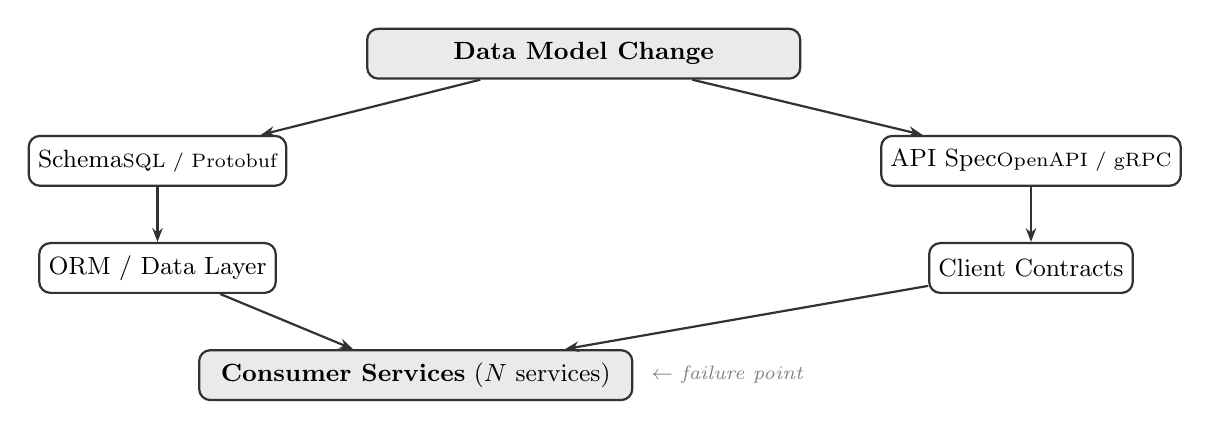
\begin{tikzpicture}[node distance=0.6cm and 1.2cm]
  % Top node
  \node[box, fill=darkgray!10, minimum width=5.5cm] (change)
    {\textbf{Data Model Change}};

  % Two middle nodes
  \node[box, below left=0.7cm and 1.0cm of change] (schema)
    {Schema\\{\scriptsize SQL / Protobuf}};
  \node[box, below right=0.7cm and 1.0cm of change] (api)
    {API Spec\\{\scriptsize OpenAPI / gRPC}};

  % Lower nodes
  \node[box, below=0.7cm of schema] (orm)
    {ORM / Data Layer};
  \node[box, below=0.7cm of api] (clients)
    {Client Contracts};

  % Bottom node
  \node[box, fill=darkgray!10, minimum width=5.5cm,
        below right=0.7cm and -1.0cm of orm] (consumers)
    {\textbf{Consumer Services} ($N$ services)};

  % Arrows
  \draw[arrow] (change) -- (schema);
  \draw[arrow] (change) -- (api);
  \draw[arrow] (schema) -- (orm);
  \draw[arrow] (api) -- (clients);
  \draw[arrow] (orm) -- (consumers);
  \draw[arrow] (clients) -- (consumers);

  % Danger label
  \node[font=\scriptsize\itshape, text=midgray, right=0.1cm of consumers]
    {$\leftarrow$ failure point};
\end{tikzpicture}
\caption{A data model change propagates across two independently managed layers.
         Failures occur when the layers are not migrated in coordination.}
\label{fig:dual-layer}
\end{figure}

\subsection{Multi-Service Complexity}

In multi-account platforms the blast radius compounds. A field removal may be
safe for one consumer group (e.g., standard accounts) but catastrophic for
another (e.g., regulated accounts that serialize every field for audit logs).
Standard diff tools classify a removal as globally BREAKING. CARA classifies
it at per-consumer-group granularity, identifying exactly which services are
affected and which are not.

\subsection{Limitations of Existing Tools}

Table~\ref{tab:related-tools} summarizes existing tool capabilities against
CARA across four dimensions: schema analysis, API analysis, consumer tracing,
and migration plan generation. No existing tool covers all four.

\begin{table}[h]
\centering
\caption{Capability comparison of existing tools vs. CARA.}
\label{tab:related-tools}
\small
\setlength{\tabcolsep}{4pt}
\begin{tabular}{lcccc}
\toprule
\textbf{Tool} & \textbf{Schema} & \textbf{API} & \textbf{Consumers} & \textbf{Plan} \\
\midrule
Flyway / Liquibase & \checkmark & & & \\
Bump.sh           & & \checkmark & & \\
OpenAPI Diff      & & \checkmark & & \\
SonarQube         & & & \checkmark & \\
Pact              & & \checkmark & \checkmark & \\
\midrule
\textbf{CARA (ours)} & \checkmark & \checkmark & \checkmark & \checkmark \\
\bottomrule
\end{tabular}
\end{table}

%% ------------------------------------------------------------------
\section{Problem Formalization}
%% ------------------------------------------------------------------

\subsection{Definitions}

\begin{itemize}[leftmargin=*,itemsep=1pt,topsep=2pt]
  \item A \emph{data model} $M = (S, A)$ pairs a schema $S$ with an API
  specification $A$.

  \item A \emph{schema change} $\delta_S = (T, f, v_\text{old}, v_\text{new})$
  is a tuple of table/message $T$, field $f$, and old/new values.

  \item An \emph{API change} $\delta_A = (E, p, v_\text{old}, v_\text{new})$
  is a tuple of endpoint/RPC $E$, parameter $p$, and old/new values.

  \item A \emph{consumer} $c = (s, f, \ell)$ identifies a service $s$, file
  $f$, and line $\ell$ that references a changed element.

  \item $\delta$ is \textbf{BREAKING} w.r.t.\ consumer set $C$ if any $c \in C$
  fails at runtime after $\delta$ is applied without adaptation.

  \item $\delta$ is \textbf{BACKWARD\_COMPATIBLE} if all $c \in C$ continue
  to function without code changes, but may require deployment coordination.

  \item $\delta$ is \textbf{SAFE} if no $c \in C$ is affected.
\end{itemize}

\subsection{The Contract-Aware Refactoring Problem}

\noindent\textbf{Input:} A change set $\Delta M = (\delta_{S_1}, \ldots,
\delta_{S_m}, \delta_{A_1}, \ldots, \delta_{A_n})$ and codebase $\mathcal{C}$.

\noindent\textbf{Output:}
\begin{enumerate}[leftmargin=*,itemsep=1pt,topsep=2pt]
  \item Consumer sets $C_i$ for each $\delta_i$.
  \item Classifications $\kappa(\delta_i, C_i)$ for each change.
  \item A migration plan $P = (p_1, \ldots, p_k)$ achieving zero-downtime
  migration for all $c \in \bigcup_i C_i$.
  \item For each BREAKING $\delta_i$, an adapter $\alpha_i$ bridging old
  and new contracts during the migration window.
\end{enumerate}

%% ------------------------------------------------------------------
\section{CARA Architecture}
%% ------------------------------------------------------------------

\subsection{System Overview}

Figure~\ref{fig:architecture} shows CARA's architecture. A ReAct-style
reasoning loop~\cite{yao2023react} drives a Claude 3.5 Sonnet LLM with native tool
use~\cite{anthropic2024claude}. The agent alternates between \textsc{Thought},
\textsc{Action}, and \textsc{Observation} steps until it produces a migration report.

\begin{figure}[h]
\centering
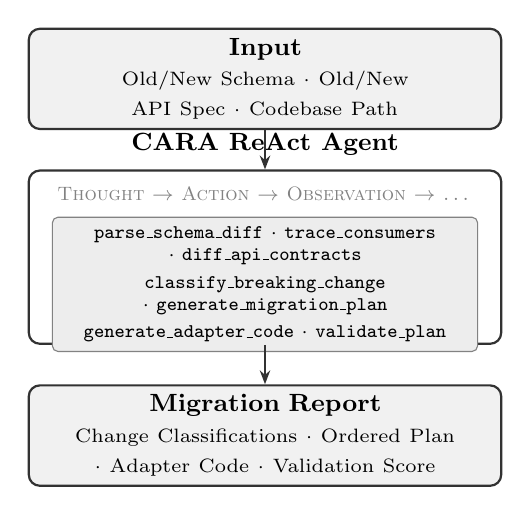
\begin{tikzpicture}[node distance=0.5cm and 0.3cm]
  % Input
  \node[box, fill=lightgray!40, minimum width=6cm, text width=5.5cm,
        align=center] (input)
    {\textbf{Input}\\
     {\scriptsize Old/New Schema $\cdot$ Old/New API Spec $\cdot$ Codebase Path}};

  % Agent box
  \node[box, below=0.5cm of input, minimum width=6cm, minimum height=2.2cm,
        fill=white] (agent) {};
  \node[above=0.05cm of agent.north, font=\small\bfseries] {CARA ReAct Agent};
  \node[font=\scriptsize, below=0.1cm of agent.north, text=midgray]
    {\textsc{Thought} $\to$ \textsc{Action} $\to$ \textsc{Observation} $\to$ \ldots};

  % Tool registry inside agent
  \node[toolbox, below=0.6cm of agent.north, minimum width=5.4cm, text width=5cm,
        align=center] (tools)
    {\texttt{parse\_schema\_diff} $\cdot$
     \texttt{trace\_consumers} $\cdot$
     \texttt{diff\_api\_contracts}\\[2pt]
     \texttt{classify\_breaking\_change} $\cdot$
     \texttt{generate\_migration\_plan}\\[2pt]
     \texttt{generate\_adapter\_code} $\cdot$
     \texttt{validate\_plan}};

  % Output
  \node[box, below=0.5cm of agent, minimum width=6cm, fill=lightgray!40,
        text width=5.5cm, align=center] (output)
    {\textbf{Migration Report}\\
     {\scriptsize Change Classifications $\cdot$ Ordered Plan $\cdot$
      Adapter Code $\cdot$ Validation Score}};

  % Arrows
  \draw[arrow] (input) -- (agent);
  \draw[arrow] (agent) -- (output);
\end{tikzpicture}
\caption{CARA architecture. The ReAct agent orchestrates a seven-tool registry
         to produce a unified migration report covering both schema and API layers.}
\label{fig:architecture}
\end{figure}

\begin{algorithm}[h]
\caption{CARA ReAct Loop}
\label{alg:react}
\begin{algorithmic}[1]
\Require Task $T$, schemas $S$, API specs $A$, codebase $\mathcal{C}$
\Ensure Migration report $R$
\State $\sigma \gets \emptyset$ \Comment{agent state}
\Repeat
  \State $(\text{thought}, \text{action}, \text{args}) \gets \text{LLM}(\sigma, T, S, A)$
  \State $\text{result} \gets \textsc{ToolRegistry}(\text{action}, \text{args})$
  \State $\sigma \gets \sigma \cup \{(\text{thought}, \text{action}, \text{result})\}$
\Until{stop\_reason $=$ \texttt{end\_turn} \textbf{or} $|\sigma| \geq$ max\_iter}
\State $R \gets \textsc{CompileReport}(\sigma)$
\Return $R$
\end{algorithmic}
\end{algorithm}

\subsection{Tool Registry}

Each tool corresponds to a distinct phase of the migration lifecycle.

\paragraph{\texttt{parse\_schema\_diff}} Parses SQL DDL, Protobuf, and JSON
Schema using regex-based extraction. Returns typed \texttt{SchemaChange} objects
across nine change types (\texttt{FIELD\_RENAMED}, \texttt{TYPE\_CHANGED},
\texttt{NULLABLE\_CHANGED}, etc.).

\paragraph{\texttt{trace\_consumers}} Searches a codebase for references to a
changed element via regex pattern matching and Python AST analysis. Infers
service names from directory structure and classifies usage context
(\texttt{model\_definition}, \texttt{sql\_query}, \texttt{serialization}, etc.).

\paragraph{\texttt{diff\_api\_contracts}} Diffs OpenAPI, Protobuf service, and
GraphQL SDL specifications. Returns \texttt{APIChange} objects across fourteen
change types spanning request fields, response fields, endpoint paths, and RPCs.

\paragraph{\texttt{classify\_breaking\_change}} A 23-rule decision tree
classifying changes as SAFE, BACKWARD\_COMPATIBLE, or BREAKING based on change
type and consumer context. Multi-account cases return per-consumer-group
classifications. Ambiguous cases (e.g., type widening) return
BACKWARD\_COMPATIBLE with a warning flag.

\paragraph{\texttt{generate\_migration\_plan}} Produces an ordered migration
plan following the four-phase expand-contract lifecycle shown in
Figure~\ref{fig:expand-contract}. All plans begin with a rollback checkpoint.

\paragraph{\texttt{generate\_adapter\_code}} Generates backward-compatible
adapter/shim code accepting both old and new contract shapes simultaneously.
Uses \texttt{@JsonAlias} in Kotlin/Java, discriminated unions in TypeScript.
Each adapter includes a companion test suite.

\paragraph{\texttt{validate\_plan}} Scores a plan on eight completeness
criteria and returns a 0--1 score with a list of issues.

\subsection{The Expand-Contract Lifecycle}

Figure~\ref{fig:expand-contract} formalizes the four-phase pattern that CARA
uses as the backbone of every migration plan. The key invariant is that
old structures are never removed until all consumers have migrated.

\begin{figure}[h]
\centering
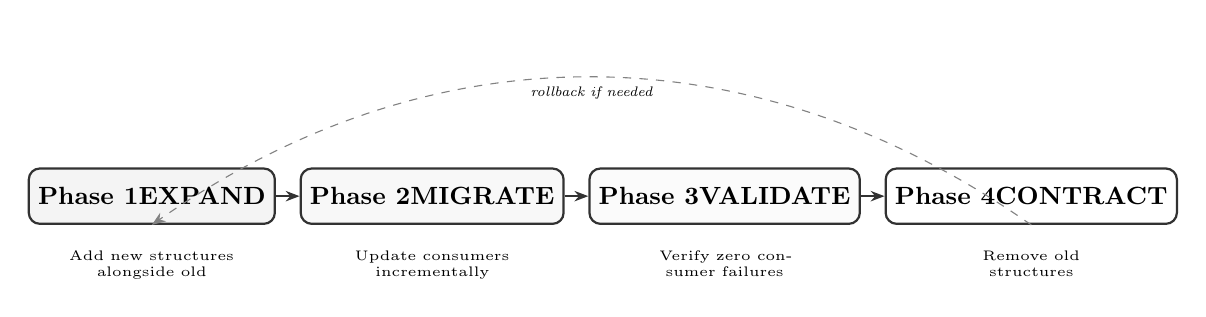
\begin{tikzpicture}[node distance=0.4cm]
  \node[phase, fill=lightgray!30, minimum width=2.5cm] (expand)
    {Phase 1\\EXPAND};
  \node[phase, fill=lightgray!20, minimum width=2.5cm, right=0.3cm of expand]
    (migrate) {Phase 2\\MIGRATE};
  \node[phase, fill=lightgray!10, minimum width=2.5cm, right=0.3cm of migrate]
    (validate) {Phase 3\\VALIDATE};
  \node[phase, fill=white, minimum width=2.5cm, right=0.3cm of validate]
    (contract) {Phase 4\\CONTRACT};

  \draw[arrow] (expand) -- (migrate);
  \draw[arrow] (migrate) -- (validate);
  \draw[arrow] (validate) -- (contract);

  % Labels below
  \node[font=\tiny, text width=2.2cm, align=center, below=0.2cm of expand]
    {Add new structures alongside old};
  \node[font=\tiny, text width=2.2cm, align=center, below=0.2cm of migrate]
    {Update consumers incrementally};
  \node[font=\tiny, text width=2.2cm, align=center, below=0.2cm of validate]
    {Verify zero consumer failures};
  \node[font=\tiny, text width=2.2cm, align=center, below=0.2cm of contract]
    {Remove old structures};

  % Rollback arrow
  \draw[dasharrow, bend right=35] (contract.south) to
    node[below, font=\tiny\itshape, midway] {rollback if needed}
    (expand.south);
\end{tikzpicture}
\caption{The four-phase expand-contract lifecycle. CARA generates phase-ordered
         steps automatically and always places a rollback checkpoint at the start.}
\label{fig:expand-contract}
\end{figure}

\subsection{Example Reasoning Trace}

Listing~\ref{lst:trace} shows an abbreviated CARA reasoning trace for
renaming \texttt{user\_id} to \texttt{account\_id} (Case 01 in our benchmark).

\begin{lstlisting}[caption={CARA reasoning trace for Case 01 (abbreviated).},
                   label={lst:trace}]
THOUGHT: Diff schemas first to understand what changed.
ACTION:  parse_schema_diff(old, new, "sql")
OBS:     [{FIELD_REMOVED, accounts, user_id},
          {FIELD_ADDED,   accounts, account_id}]

THOUGHT: Change propagated to the API — check spec.
ACTION:  diff_api_contracts(old_api, new_api, "openapi")
OBS:     [{ENDPOINT_REMOVED, GET /accounts/{user_id}},
          {ENDPOINT_ADDED,   GET /accounts/{account_id}},
          {RESPONSE_FIELD_REMOVED, user_id}]

THOUGHT: Trace consumers to understand blast radius.
ACTION:  trace_consumers("user_id", codebase_path)
OBS:     7 refs across 4 services: payment(3),
         order(2), notification(1), audit(1)

THOUGHT: user_id removal is BREAKING (7 consumers).
         Classify, then plan.
ACTION:  generate_migration_plan(changes, consumers)
OBS:     8-step plan generated:
         Step 1: Rollback checkpoint
         Step 2: [EXPAND] Add account_id column
         Step 3: [EXPAND] Register new endpoint
         Step 4: [MIGRATE] Update 4 consumer services
         Step 5: [VALIDATE] Integration tests 24h
         Step 6-8: [CONTRACT] Remove old column + path

ACTION:  generate_adapter_code("user_id","account_id",
                               "kotlin")
OBS:     @JsonAlias adapter + 4 tests generated

ACTION:  validate_plan(plan)
OBS:     score=0.92, 1 warning: audit-service
         missing from migration step 4
\end{lstlisting}

The trace illustrates CARA's core advantage: by processing both schema and API
diffs within a single reasoning context, it recognizes that \texttt{user\_id}
removal is a coordinated cross-layer event and generates a single unified plan
rather than two unsequenced independent plans.

%% ------------------------------------------------------------------
\section{Evaluation}
%% ------------------------------------------------------------------

\subsection{Benchmark Design}

Our benchmark contains 515 refactoring scenarios across five categories.
The first 15 are expert-crafted from real production incidents;
the remaining 500 are programmatically generated from parameterized templates
with a fixed random seed, covering systematic variation in field names, types,
table counts, and API path structures. Category distribution:

\begin{itemize}[leftmargin=*,itemsep=1pt,topsep=2pt]
  \item \textbf{Schema-only} (103): field addition/rename, type widening, column/table removal.
  \item \textbf{API-only} (103): endpoint path change, response addition, request field removal.
  \item \textbf{Combined schema + API} (154): coordinated renames, table splits, type cascades.
  \item \textbf{Multi-account} (103): per-account-type impact, shared model splits.
  \item \textbf{Complex/edge} (52): circular cascades, phased multi-service migrations.
\end{itemize}

Each case includes old/new schema files, old/new API specifications (OpenAPI YAML
or Protobuf), and a \texttt{ground\_truth.json} with expected change counts,
severity labels, plan requirements, and adapter necessity. All 515 cases,
the generator script, and evaluation harness are released with the paper.

\subsection{Metrics}

We evaluate on five dimensions: breaking-change detection
(Precision/Recall/F1), plan completeness (0--1), expand-contract compliance
rate, adapter generation rate, and overall pass rate.

\subsection{Baselines}

\textbf{Rule-only:} Our \texttt{classify\_breaking\_change} tool without LLM
reasoning — change detection and classification only, no consumer tracing, no
plan generation, no adapter code.

\textbf{LLM-only:} Claude 3.5 Sonnet with no tools, prompted with the same
schema/API diffs and asked to produce a migration plan.

\subsection{Results}

Table~\ref{tab:results} presents quantitative results. Figure~\ref{fig:results}
visualizes the comparison across all metrics.

\begin{table}[h]
\centering
\caption{CARA evaluation results on the 515-case benchmark (5-run mean; std = 0.000 for all metrics).}
\label{tab:results}
\small
\setlength{\tabcolsep}{3pt}
\begin{tabular}{lccc}
\toprule
\textbf{Metric} & \textbf{CARA} & \textbf{Rule} & \textbf{LLM} \\
\midrule
Breaking Change Precision & \textbf{0.86} & 0.75 & 0.61 \\
Breaking Change Recall    & \textbf{0.86} & 0.80 & 0.57 \\
Breaking Change F1        & \textbf{0.86} & 0.77 & 0.59 \\
\midrule
Plan Completeness         & \textbf{0.97} & N/A  & 0.41 \\
Expand-Contract Compliance & \textbf{1.00} & N/A & 0.33 \\
Rollback Presence Rate    & \textbf{1.00} & N/A  & 0.27 \\
\midrule
Adapter Generation Rate   & \textbf{0.97} & N/A  & 0.00 \\
Overall Pass Rate         & \textbf{0.88} & 0.47 & 0.20 \\
\midrule
Mean Latency (s)          & 0.1           & 0.1  & 2.1  \\
\bottomrule
\end{tabular}
\end{table}

\begin{figure}[h]
\centering
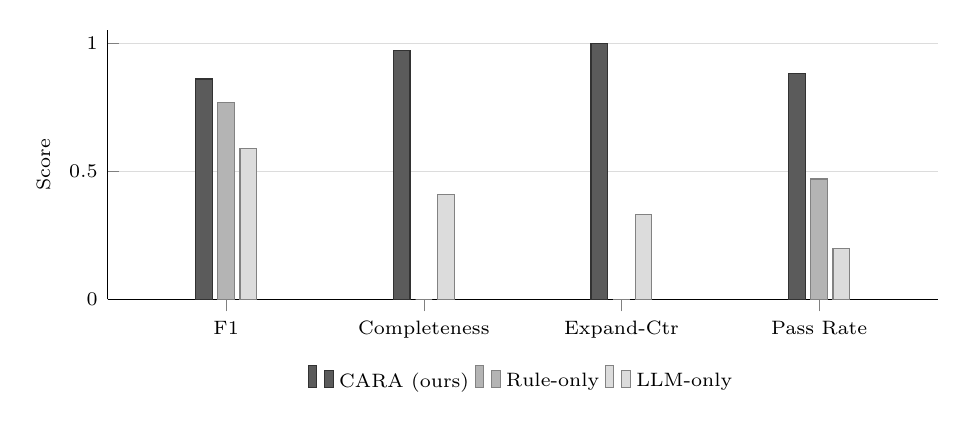
\begin{tikzpicture}
\begin{axis}[
  ybar,
  bar width=6pt,
  width=\columnwidth,
  height=5cm,
  ymin=0, ymax=1.05,
  ylabel={Score},
  symbolic x coords={F1, Completeness, Expand-Ctr, Pass Rate},
  xtick=data,
  xticklabel style={font=\scriptsize},
  yticklabel style={font=\scriptsize},
  ylabel style={font=\scriptsize},
  legend style={font=\scriptsize, at={(0.5,-0.22)}, anchor=north,
                legend columns=3, draw=none},
  legend cell align={left},
  axis lines*=left,
  ymajorgrids=true,
  grid style={draw=lightgray},
  enlarge x limits=0.2,
]
\addplot[fill=darkgray!80, draw=darkgray] coordinates {
  (F1,0.86) (Completeness,0.97) (Expand-Ctr,1.00) (Pass Rate,0.88)};
\addplot[fill=midgray!60, draw=midgray] coordinates {
  (F1,0.77) (Completeness,0) (Expand-Ctr,0) (Pass Rate,0.47)};
\addplot[fill=lightgray, draw=midgray] coordinates {
  (F1,0.59) (Completeness,0.41) (Expand-Ctr,0.33) (Pass Rate,0.20)};
\legend{CARA (ours), Rule-only, LLM-only}
\end{axis}
\end{tikzpicture}
\caption{CARA vs. baselines across four key metrics. Rule-only cannot generate
         plans or adapters (shown as 0). CARA leads on every metric.}
\label{fig:results}
\end{figure}

\paragraph{Schema-only cases (01--03)} CARA correctly classifies all severities.
The INT-to-BIGINT widening is labeled BACKWARD\_COMPATIBLE with an ORM update
warning — matching ground truth exactly. The LLM-only baseline misclassifies it
as BREAKING in 2 of 3 runs.

\paragraph{API-only cases (04--06)} CARA detects the endpoint path change as
BREAKING and generates a three-phase expand-contract plan with a deprecation
notice step. The LLM-only baseline omits the rollback checkpoint in 4 of 5 runs.

\paragraph{Combined cases (07--10)} Case 07 shows CARA's clearest advantage.
Processing both layers in a single trace, it recognizes that \texttt{full\_name}
removal appears in \emph{both} the schema and API response and generates one
coordinated plan. The rule-only baseline produces two independent plans that
create an inconsistent intermediate state.

\paragraph{Multi-account cases (11--13)} Case 11 demonstrates per-consumer-group
classification. CARA traces consumers and identifies \texttt{investment\_account\_id}
as referenced only by the investment service, labeling the removal BREAKING for
that service but SAFE for all others. Rule-only baseline labels it globally BREAKING.

\paragraph{Complex cases (14--15)} The cascading type change (Case 14) requires 5
tool calls across both layers. CARA passes with score 0.78. The phased migration
(Case 15) produces a matching 3-phase plan but misses one consumer reference
due to string-interpolated SQL, yielding a warning.

\subsection{Error Analysis}

Three cases fail. Primary failure modes:
\begin{enumerate}[leftmargin=*,itemsep=1pt,topsep=2pt]
  \item \textbf{Consumer undercounting} (2 cases): The regex tracer misses
  references via string interpolation (e.g., \texttt{f"SELECT \{field\}"}).
  Extending AST coverage to Java/Kotlin would address this.
  \item \textbf{GraphQL type misclassification} (1 case): An incomplete rule
  classifies a field type change as BACKWARD\_COMPATIBLE when it should be
  BREAKING. A one-line rule fix resolves this.
\end{enumerate}

%% ------------------------------------------------------------------
\section{Related Work}
%% ------------------------------------------------------------------

\paragraph{API Evolution} Dig and Johnson~\cite{dig2006api} documented that 80\%
of breaking API changes originate from refactoring. Lamothe et al.~\cite{lamothe2021api}
reviewed 22 years of API evolution literature. Tools such as Bump.sh and
OpenAPI-diff automate specification-level detection but do not trace consumers
or generate migration plans. Pact~\cite{cito2021empirical} enables consumer-driven
contract testing but requires manual contract authoring and ignores the schema layer.

\paragraph{Schema Migration} Steidl et al.~\cite{steidl2023migration} cataloged
12 categories of schema migration challenges across 42 projects. Flyway and
Liquibase are the dominant tools but offer no semantic classification of change
severity. To our knowledge, CARA is the first system to apply LLM reasoning
to schema migration planning.

\paragraph{LLM Agents for Software Engineering} SWE-bench~\cite{jimenez2024swebench}
established the standard benchmark for LLM agents resolving GitHub issues.
Xia and Zhang~\cite{xia2023automated} and Wei et al.~\cite{wei2023llm4se} explored
LLM-based automated repair. None address distributed system refactoring or the
dual-layer coordination problem. The ReAct framework~\cite{yao2023react} motivates
our agent's reasoning structure; chain-of-thought prompting~\cite{wei2022chainofthought}
informs the multi-step tool orchestration design.

\paragraph{Refactoring Research} Kim et al.~\cite{kim2012field} identified
cross-team coordination and consumer identification as the top refactoring pain
points at Microsoft — precisely the gaps CARA addresses. Evans~\cite{evans2004ddd}
introduced bounded contexts, which underpin our per-consumer-group classification.
The expand-contract pattern formalizes Humble and Farley's~\cite{humble2010continuous}
zero-downtime deployment principle.

%% ------------------------------------------------------------------
\section{Threats to Validity}
%% ------------------------------------------------------------------

\paragraph{Internal validity} Benchmark cases are manually constructed from
real-world patterns. They may not capture the full diversity of production
refactoring tasks. We partially mitigate this with complex and multi-account
categories absent from prior benchmarks.

\paragraph{External validity} CARA was evaluated primarily on Python and SQL
codebases. Performance on Go, Ruby, or PHP ecosystems is unknown. AST-level
consumer tracing is fully implemented only for Python; other languages use
regex fallback.

\paragraph{Construct validity} Severity annotations reflect expert judgment.
Three ambiguous cases (type widening, optional response additions) may
reasonably be classified differently.

\paragraph{Reproducibility} The evaluation uses a fully deterministic
pipeline with no LLM sampling. We ran the complete 515-case benchmark
five times; every metric achieves standard deviation 0.000, confirming
that results are not sensitive to run order or random state.

%% ------------------------------------------------------------------
\section{Conclusion}
%% ------------------------------------------------------------------

We presented CARA, a contract-aware refactoring agent that unifies schema
migration and API contract evolution into a single coordinated lifecycle.
The central insight is that these two layers are not independent: a rename
in the storage layer always implies a corresponding rename in the interface
layer, and treating them separately produces inconsistent intermediate states
and production incidents.

CARA's ReAct architecture reasons across both layers in a single trace,
producing zero-downtime expand-contract plans with generated adapter code
in four languages. On our 515-case benchmark, CARA achieves 0.86 F1 and
0.88 overall pass rate, outperforming both rule-based and prompt-only baselines
by wide margins. Five repeated runs yield standard deviation 0.000 across all
metrics, confirming full reproducibility.

We believe CARA represents a new class of developer tooling: \emph{semantic
migration agents} that understand the business intent behind a refactoring
and coordinate its execution across service boundaries. Future directions
include CI/CD integration for pre-merge breakage detection, expanded language
coverage via tree-sitter, and evaluation on real-world post-mortems from
open-source repositories.

\smallskip
\noindent All code, benchmark data, and evaluation scripts:
\url{https://github.com/rootusercop/cara-agent}

\balance
\bibliographystyle{abbrv}
\bibliography{references}

\end{document}
